%!Tex Root = ../content_Linux_Installation.tex
% ./content_Linux_Installation/Design
% ./content_Linux_Installation/Deklarationen
% ./content_Linux_Installation/Before_Installation
% ./content_Linux_Installation/Base_Installation
% ./content_Linux_Installation/After_Base_Installation

% https://tex.stackexchange.com/questions/83101/option-clash-for-package-xcolor
% [table]
% https://tex.stackexchange.com/questions/14336/latex-beamer-presentation-package-169-aspect-ratio
% https://tex.stackexchange.com/questions/203045/latex-error-option-clash-for-package-hyperref
% https://stackoverflow.com/questions/3637129/how-can-i-top-align-the-content-of-a-fragile-frame-in-a-latex-beamer-presentat
% https://latex-beamer.com/faq/place-content-frame/
\documentclass[aspectratio=169, hyperref={colorlinks=true, allcolors=PrimaryColor}, c]{beamer}

% \usepackage[margin=1.5cm, headheight=12.5pt]{geometry}
\usepackage[ngerman]{babel}

\usepackage{lipsum}

\usepackage[parfill]{parskip}
% % https://latexref.xyz/bs-par.html
\setlength{\parskip}{0.4cm} % space between paragraphs
% \usepackage{setspace}

% as beamer itself already provides these functionalities, there is no need to load hyperref, color, graphicx, graphics
% \usepackage{graphicx}

% % https://tex.stackexchange.com/questions/48509/insert-list-of-figures-in-the-table-of-contents
% \usepackage[nottoc]{tocbibind}

% % colorbox stuff
\usepackage{tcolorbox}
\usepackage{tikz}
\usetikzlibrary {arrows.meta,positioning}
\usetikzlibrary{graphs}
\tcbuselibrary{skins}
\tcbuselibrary{breakable}
\usetikzlibrary{patterns}
\usetikzlibrary{shadings}
\tcbuselibrary{theorems}
% \tcbuselibrary{listings}
% https://tex.stackexchange.com/questions/550052/command-parboxrestore-has-changed
\tcbuselibrary{minted}
\tcbset{listing engine=minted}
\tcbuselibrary{raster}

% % https://tex.stackexchange.com/questions/547950/highlight-labeled-lines-of-code-with-minted
% % \usepackage{refcount}

% \usepackage{cleveref}

\usepackage[style=authortitle]{biblatex}
\addbibresource{./My Library/My Library.bib}

% \usepackage{pdfpages}
% https://tex.stackexchange.com/questions/94845/problems-with-toprule-and-midrule-in-a-table

\usepackage{booktabs} % for table rules
% % \usepackage{tabulary}
% % https://tex.stackexchange.com/questions/395554/command-rowcolors-from-colortbl-does-not-work-as-expected

\usepackage{nicematrix}
% \usepackage{tabularx}
% \usepackage{array}
% \usepackage{multirow}
% \usepackage{amssymb}

% https://tex.stackexchange.com/questions/157389/how-to-center-column-values-in-a-table
% \newcolumntype{P}[1]{>{\centering\arraybackslash}p{#1}}

% https://stackoverflow.com/questions/2888817/footnotes-for-tables-in-latex
% \usepackage{tablefootnote}

% https://tex.stackexchange.com/questions/8625/force-figure-placement-in-text
% \usepackage{float}

% https://tex.stackexchange.com/questions/219445/line-break-in-texttt
\usepackage{seqsplit}
\newcommand{\seqtt}[1]{{\scriptsize\texttt{\seqsplit{#1}}}}
\newcommand{\smalltt}[1]{{\small\texttt{#1}}}
\newcommand{\tinytt}[1]{{\tiny\texttt{#1}}}
\newcommand{\scripttt}[1]{{\scriptsize\texttt{#1}}}

% https://tex.stackexchange.com/questions/358292/creating-a-subcounter-to-a-counter-i-created
\usepackage{chngcntr}

% https://tex.stackexchange.com/questions/18870/defining-an-new-itemize-like-environment-where-itemfoo-passes-foo-to-a-macro
\usepackage{ifmtarg}


% https://stackoverflow.com/questions/1061112/eliminate-space-before-beginitemize
% https://tex.stackexchange.com/questions/31505/trouble-combining-enumitem-and-beamer
% https://tex.stackexchange.com/questions/325003/given-enumitem-beamer-incompatibility-how-do-i-adjust-the-indent-of-the-enume
% https://tex.stackexchange.com/questions/455692/beamer-presentation-with-itemize-exceed-text-capacity
% \usepackage{enumitem}

% https://tex.stackexchange.com/a/263470
\usepackage{microtype}

% https://tex.stackexchange.com/questions/165178/nameref-hyperref-evaluating-counter-instead-of-section-name
% \usepackage{nameref}

% https://stackoverflow.com/questions/1078370/subfigs-of-a-figure-on-multiple-pages
% \usepackage{subfig}

% https://tex.stackexchange.com/questions/186981/is-there-a-subsubsubsection-command
% https://tex.stackexchange.com/questions/130795/how-can-i-number-sections-below-subsection-in-latex
% \setcounter{secnumdepth}{5}

% % https://stackoverflow.com/questions/2854299/getting-subsection-to-list-in-table-of-contents-in-latex
\setcounter{tocdepth}{4}

% https://tex.stackexchange.com/questions/369421/how-to-have-a-figure-going-over-several-pages
% TODO: set hypcap = true when compiling for the last time
% https://tex.stackexchange.com/questions/132611/change-color-of-figure-caption-text
\usepackage[labelfont={color=SecondaryColor, it}, textfont={it}]{caption}
% hypcap=false

% https://tex.stackexchange.com/questions/7210/label-and-caption-without-float
\DeclareCaptionType{codecaption}[Code][Codeverzeichnis]
% https://tex.stackexchange.com/questions/449677/spaces-in-newenvironment
\newenvironment{code}{\bigskip\captionsetup{type=codecaption}}{\medskip}

% https://texblog.net/latex-archive/uncategorized/prevent-floating-image-figure-table/
% \newcommand\captionof[1]{\def\@captype{#1}\caption}
% \usepackage{capt-of}

% \usepackage{formal-grammar}

% newfloat package
% \SetupFloatingEnvironment{floatgrammar}{name=Grammatik}

% \renewcommand{\downplay}[0]{\rowstyle{\color{gray!90!black}}}
% \newcommand{\removed}[0]{\rowstyle{\color{red}}}

% https://tex.stackexchange.com/questions/26637/how-do-you-get-mathbb1-to-work-characteristic-function-of-a-set
% \usepackage{bbm}
% \usepackage{newtxmath}

% https://tex.stackexchange.com/questions/27843/level-of-boldness-changeable
\usepackage[bold=1]{xfakebold}

% \newcommand{\footnoteurl}[1]{\href{#1}{Link}\footnote{\url{#1}.}}

% https://www.namsu.de/Extra/befehle/Cases.html
\usepackage{mathtools}

\usepackage{breqn}

% https://tex.stackexchange.com/questions/479632/newcommand-combine-optional-star-and-optional-parameter
% \usepackage{xparse}
\tcbuselibrary{xparse}

% https://texfaq.org/FAQ-twooptarg
\usepackage{xargs}

\newenvironmentx{transformation}[3][1=0.3, 2=0.2, 3=0.4]{
  \newcommand{\compilesto}{%
    \end{column}\begin{column}{#2\linewidth}\centering$\Rightarrow$\end{column}\begin{column}{#3\linewidth}\centering}
  \newcommand{\arrowx}[1]{%
    \end{column}\begin{column}{#2\linewidth}\centering$\xRightarrow{##1}$\end{column}\begin{column}{#3\linewidth}\centering}
  \newcommand{\arrowxx}[2]{%
    \end{column}\begin{column}{#2\linewidth}\centering$\xRightarrow[##2]{##1}$\end{column}\begin{column}{#3\linewidth}\centering}
  \begin{columns}\begin{column}{#1\linewidth}\centering
  }{%
  \end{column}\end{columns}%
}

% emojis
% \usepackage{tikzsymbols}

% \usepackage[german]{algorithm2e}

% https://tex.stackexchange.com/questions/237974/hide-section-numbering-but-keep-labeling
% reference titles of sections
% \usepackage[usetoc]{titleref}

% % https://tex.stackexchange.com/questions/531/what-is-the-best-way-to-use-quotation-mark-glyphs
\usepackage{csquotes}

% https://tex.stackexchange.com/questions/326527/colored-blocks-for-numbered-theorems-in-beamer
\usepackage{etoolbox}% new package to be loaded

% https://jansoehlke.com/2010/06/strikethrough-in-latex/
\usepackage[normalem]{ulem}
% \usepackage{cancel}

%!Tex Root = ../content_Linux_Installation.tex
% ./content_Linux_Installation/Packete
% ./content_Linux_Installation/Deklarationen
% ./content_Linux_Installation/Before_Installation
% ./content_Linux_Installation/Base_Installation
% ./content_Linux_Installation/After_Base_Installation

% ┌──────────────────────┐
% │ Beamer Configuration │
% └──────────────────────┘

\usetheme{default}
\useoutertheme{infolines}

% ┌─────────────────────┐
% │ Color Configuration │
% └─────────────────────┘

% % https://latexdraw.com/how-to-draw-venn-diagrams-in-latex/
% as beamer itself already provides these functionalities, there is no need to load hyperref, color, graphicx, graphics
% \usepackage{xcolor}
\definecolor{PrimaryColor}{HTML}{2a8892}
\definecolor{PrimaryColorDimmed}{HTML}{a8dec5}
\definecolor{SecondaryColor}{HTML}{e96e1a}
\definecolor{SecondaryColorDimmed}{HTML}{FCBB69}
\colorlet{BoxColor}{gray!10!white}

\setbeamercolor{normal text}{%
  fg=black,
  bg=white
}
\setbeamercolor{alerted text}{%
  fg=SecondaryColor,
}

% \setbeamercolor{example text}{%
%   fg=PrimaryColor,
% }

\setbeamercolor{structure}{fg=SecondaryColor}

\setbeamercolor{frametitle}{fg=PrimaryColor}
\setbeamercolor{framesubtitle}{fg=SecondaryColor}

\setbeamercolor{title}{fg=PrimaryColor, bg=BoxColor}
\setbeamercolor{subtitle}{fg=SecondaryColor}

% https://github.com/josephwright/beamer/blob/main/base/themes/color/beamercolorthemedefault.sty
% https://github.com/josephwright/beamer/blob/main/base/themes/outer/beamerouterthemeinfolines.sty
\setbeamercolor{author in head/foot}{fg=PrimaryColor, bg=PrimaryColorDimmed}
\setbeamercolor{title in head/foot}{fg=SecondaryColor, bg=SecondaryColorDimmed}
\setbeamercolor{date in head/foot}{fg=PrimaryColor, bg=PrimaryColorDimmed}

\setbeamercolor{palette primary}{fg=PrimaryColor,bg=PrimaryColorDimmed}
\setbeamercolor{palette secondary}{fg=SecondaryColor,bg=SecondaryColorDimmed}
\setbeamercolor{palette tertiary}{fg=PrimaryColor,bg=PrimaryColorDimmed}
\setbeamercolor{palette quaternary}{fg=PrimaryColor,bg=PrimaryColorDimmed}

\setbeamercolor{block title}{fg=white, bg=PrimaryColor}
\setbeamercolor{block body}{fg=black, bg=BoxColor}

\setbeamercolor{block title example}{fg=white, bg=PrimaryColor}
\setbeamercolor{block body example}{fg=black, bg=BoxColor}

\setbeamercolor{block title alerted}{fg=white, bg=SecondaryColor}
\setbeamercolor{block body alerted}{fg=black, bg=BoxColor}

% https://tex.stackexchange.com/questions/326527/colored-blocks-for-numbered-theorems-in-beamer
% https://tex.stackexchange.com/questions/87216/how-to-change-the-color-of-the-text-in-a-theorem-in-beamer/87219#87219
\AtBeginEnvironment{theorem}{% set of commands to be added
    \setbeamercolor{block title}{fg=white,bg=PrimaryColor}% colors to change
    \setbeamercolor{block body}{fg=black,bg=PrimaryColorDimmed}% colors to change
}

\AtBeginEnvironment{proof}{%
    \setbeamercolor{block title}{fg=white,bg=SecondaryColor}
    \setbeamercolor{block body}{fg=black,bg=SecondaryColorDimmed}
}

% https://tex.stackexchange.com/questions/87133/changing-the-color-of-itemize-item-in-beamer
\setbeamercolor{itemize item}{fg=SecondaryColor}
\setbeamercolor{itemize subitem}{fg=SecondaryColor}
\setbeamercolor{itemize subsubitem}{fg=SecondaryColor}

\setbeamercolor{enumerate item}{fg=SecondaryColor}
\setbeamercolor{enumerate subitem}{fg=SecondaryColor}
\setbeamercolor{enumerate subsubitem}{fg=SecondaryColor}

% ┌─────────────────────────┐
% │ Titlepage Configuration │
% └─────────────────────────┘

\newcommand{\titlesecond}{Linux Installation}
\newcommand{\subtitlesecond}{Schritt für Schritt}
\newcommand{\type}{
  Anleitung\\[-0.25cm]
  \rule{7cm}{0.1mm}
}
\newcommand{\authorsecond}{Jürgen Mattheis}
\newcommand{\moreinformation}{
% \begin{columns}
% \begin{column}{0.5\textwidth}
%   \raggedright
%   \small
%   \emph{Weitere Aufgabe:}
%
%   Weitere Person
% \end{column}
% \begin{column}{0.5\textwidth}
%   \raggedleft
%   \small
%   \emph{Weitere Aufgabe:}
%
%   Weitere Person
% \end{column}
% \end{columns}
  \emph{Korrekturen bitte an:}\\
  \url{https://github.com/matthejue/PicoC-Compiler_Uebungsblatt/issues}.
}
\newcommand{\institutesecond}{Universität Freiburg}
\newcommand{\datesecond}{\today}
% \logo{\includegraphics[height=0.5cm]{./figures/logo.png}}

\newcommand{\lehrstuhl}{Lehrstuhl für Betriebssysteme}

\defbeamertemplate*{title page2}{default}[1][]{
  \vbox{}
  \vfill
  \begingroup
    \centering
    \begin{beamercolorbox}[sep=8pt,center,#1]{title}
      \usebeamerfont{title}\titlesecond\par%
      \ifx\subtitlesecond\@empty%
      \else%
        \vskip0.25em%
        {\usebeamerfont{subtitle}\usebeamercolor[fg]{subtitle}\subtitlesecond\par}%
      \fi%
    \end{beamercolorbox}%
    \begin{beamercolorbox}[sep=8pt,center,#1]{institute}
       \type
    \end{beamercolorbox}
    \begin{beamercolorbox}[sep=8pt,center,#1]{author}
      \usebeamerfont{author}\emph{Präsentator:}\\ \authorsecond
    \end{beamercolorbox}
    \begin{beamercolorbox}[sep=8pt,center,#1]{institute}
      \moreinformation
    \end{beamercolorbox}\vskip1em
    \begin{beamercolorbox}[sep=8pt,center,#1]{date}
      \usebeamerfont{date}\emph{\datesecond}
    \end{beamercolorbox}
    \begin{beamercolorbox}[sep=8pt,center,#1]{institute}
      \usebeamerfont{institute}\institutesecond, \lehrstuhl
    \end{beamercolorbox}
    {\usebeamercolor[fg]{titlegraphic}\inserttitlegraphic\par}
  \endgroup
  \vfill
}

\makeatletter
\def\titlepagesecond{\usebeamertemplate*{title page2}\@thanks}
\makeatother

\setbeamertemplate{title page2}[default][colsep=-4bp,rounded=true,shadow=true]

% ┌───────────────────────┐
% │ Footline and Headline │
% └───────────────────────┘

% https://github.com/josephwright/beamer/blob/main/base/themes/outer/beamerouterthemeinfolines.sty
\makeatletter
\setbeamertemplate{footline}{%
  \leavevmode%
  \hbox{%
    \begin{beamercolorbox}[wd=.333333\paperwidth,ht=2.25ex,dp=1ex,center]{author in head/foot}%
      \usebeamerfont{author in head/foot}\authorsecond % \expandafter\ifblank\expandafter{\beamer@shortinstitute}{}{~~(\insertshortinstitute)}
    \end{beamercolorbox}%
    \begin{beamercolorbox}[wd=.333333\paperwidth,ht=2.25ex,dp=1ex,center]{title in head/foot}%
      \usebeamerfont{title in head/foot}\titlesecond
    \end{beamercolorbox}%
    \begin{beamercolorbox}[wd=.333333\paperwidth,ht=2.25ex,dp=1ex,leftskip=2ex,rightskip=2ex,sep=0pt]{date in head/foot}%
      \hfill%
      \usebeamerfont{author in head/foot}%
      \institutesecond
      \hfill%
      \usebeamercolor[fg]{page number in head/foot}%
      \usebeamerfont{page number in head/foot}%
      \usebeamertemplate{page number in head/foot}%
    \end{beamercolorbox}
  }%
  \vskip0pt%
}
\makeatother

\setbeamertemplate{headline}{%
\leavevmode%
  \hbox{%
    % https://tex.stackexchange.com/questions/85439/custom-headline-in-latex-beamer
    \begin{beamercolorbox}[wd=\paperwidth,ht=2.5ex,dp=1.125ex]{palette quaternary}%
      \textcolor{PrimaryColor}{\insertsectionnavigationhorizontal{\paperwidth}{\hskip0pt plus1filll}{\hskip0pt plus1filll}}
    \end{beamercolorbox}%
  }
}

% https://tex.stackexchange.com/questions/44983/beamer-removing-headline-and-its-space-on-a-single-frame-for-plan-but-keepin
\newenvironment{withoutheadline}{
  \setbeamertemplate{headline}{%
  \leavevmode%
    \hbox{%
      \begin{beamercolorbox}[wd=\paperwidth,ht=2.5ex,dp=1.125ex]{palette primary}%
      \end{beamercolorbox}%
    }
  }
}{}

\newenvironment{withoutfootline}{
  \setbeamertemplate{footline}{%
  \leavevmode%
    \hbox{%
      \begin{beamercolorbox}[wd=\paperwidth,ht=2.5ex,dp=1.125ex]{palette secondary}%
      \end{beamercolorbox}%
    }
  }
}{}

% ┌──────────────────────┐
% │ Layout Configuration │
% └──────────────────────┘

\setbeamertemplate{blocks}[rounded][shadow=true]

% https://tex.stackexchange.com/questions/578098/number-of-figure-in-beamer
\setbeamertemplate{caption}[numbered]

% \setbeamertemplate{sidebar canvas left}{}
\setbeamersize{sidebar width right=1.5cm}
\setbeamertemplate{sidebar right}{%
  \vspace*{\fill}
  
\includegraphics[width=1.5cm]{./figures/background.png}
  \vspace*{\fill}
}

\newcommand{\insertsectionHEAD}{%
	\expandafter\insertsectionHEADaux\insertsectionhead}
	\newcommand{\insertsectionHEADaux}[3]{\LARGE#3
}

\AtBeginSection[] {
  \begingroup
  \setbeamercolor{background canvas}{bg=PrimaryColorDimmed}

  \setbeamertemplate{sidebar right}{%
    \vspace*{\fill}
    
\includegraphics[width=1.5cm]{./figures/background.png}
    \vspace*{\fill}
  }

  \begin{frame}
    \centering
    \textcolor{PrimaryColor}{\insertsectionHEAD}
  \end{frame}
  \endgroup
}

% TOC at beginning of each section
% \AtBeginSection[]{
%   \begin{frame}{Gliederung}
%     \tableofcontents[currentsection]
%   \end{frame}
% }

% https://tex.stackexchange.com/questions/87133/changing-the-color-of-itemize-item-in-beamer
\setbeamertemplate{itemize item}[triangle]
\setbeamertemplate{itemize subitem}[triangle]
\setbeamertemplate{itemize subsubitem}[triangle]
% square, circle, triangle, \rightTextArrow

% ┌────────────────────┐
% │ Font Configuration │
% └────────────────────┘

\setbeamerfont{title}{size=\LARGE}
\setbeamerfont{date}{size=\footnotesize}
\setbeamerfont{author}{size=\small}
\setbeamerfont{institute}{size=\small}
\setbeamerfont{subtitle}{size=\large}

\setbeamerfont{frametitle}{size=\LARGE}
\setbeamerfont{framesubtitle}{size=\large}

\setbeamerfont{normal text}{size=\tiny}

% ┌───────────┐
% │ Resources │
% └───────────┘

% - latex beamer templates als Inspiration: https://github.com/benjamin-weiss/hsrmbeamertheme/blob/master/beamerthemehsrm.sty
% - inspiration: https://github.com/martinbjeldbak/ultimate-beamer-theme-list
% - https://github.com/matze/mtheme
% - https://github.com/josephwright/beamer/blob/main/base/themes/color/beamercolorthemedefault.sty
  % - different templates switch
% - https://github.com/josephwright/beamer/blob/main/base/themes/color/beamercolorthemecrane.sty
% - https://github.com/josephwright/beamer/blob/main/base/themes/color/beamercolorthemebeetle.sty
% - https://www.cpt.univ-mrs.fr/~masson/latex/Beamer-appearance-cheat-sheet.pdf
% - (https://git.imp.fu-berlin.de/raup90/swp_2019/-/blob/master/presentation/fu-beamer-template.tex)

%!Tex Root = ../content_Linux_Installation.tex
% ./content_Linux_Installation/Packete
% ./content_Linux_Installation/Design
% ./content_Linux_Installation/Before_Installation
% ./content_Linux_Installation/Base_Installation
% ./content_Linux_Installation/After_Base_Installation


% ┌──────────┐
% │ Settings │
% └──────────┘

% https://tex.stackexchange.com/questions/584071/configure-minted-style-in-latex-for-code-highlighting
% https://pygments.org/docs/tokens/
% https://pygments.org/docs/styledevelopment/#creating-own-styles
% 'custom':  'custom::CustomStyle' in /usr/lib/python3.10/site-packages/pygments/styles/__init__.py
% https://tex.stackexchange.com/questions/18083/how-to-add-custom-c-keywords-to-be-recognized-by-minted#comment930474_42392
\usemintedstyle{custom}

% https://tex.stackexchange.com/questions/345976/global-settings-for-minted
\setminted{fontsize=\tiny,breaklines,highlightcolor=SecondaryColorDimmed,autogobble,escapeinside=||,breakafter={_},breakbefore={(},breakaftersymbolpre={},breakaftersymbolpost={},breakbeforesymbolpre={},breakbeforesymbolpost={},breaksymbolsepleft=2mm,breaksymbolsepright=0mm,breakindent=0mm,breaksymbolindentleft=5mm,breaksymbolindentright=0mm,numbersep=2.5mm}

\newenvironment{linenums}{
  \setminted{linenos}
}{}

% https://tex.stackexchange.com/questions/325003/given-enumitem-beamer-incompatibility-how-do-i-adjust-the-indent-of-the-enume
% https://tex.stackexchange.com/questions/455692/beamer-presentation-with-itemize-exceed-text-capacity
% \setlist[itemize]{itemsep=2mm, topsep=2mm, parsep=0mm, partopsep=0mm}

% ┌───────┐
% │ Boxes │
% └───────┘

\DeclareTCBInputListing{\codebox}{ s o m }{listing file={#3},
  enhanced,colframe=PrimaryColor,colback=BoxColor,IfBooleanTF={#1}{colframe=SecondaryColor}{colframe=PrimaryColor},fonttitle=\tiny,#2,listing only,halign title=center,drop fuzzy shadow,arc=1mm,bottom=1mm,top=1mm,left=1mm,right=1mm,boxrule=0.5mm,listing engine=minted}
% , sharpish corners

% % https://tex.stackexchange.com/questions/585582/inside-of-a-newtcbinputlisting-how-can-i-change-the-color-of-the-line-number-as
% % https://www.overleaf.com/learn/latex/Using_colours_in_LaTeX
% https://tex.stackexchange.com/questions/132849/how-can-i-change-the-font-size-of-the-number-in-minted-environment
\renewcommand{\theFancyVerbLine}{\ttfamily\textcolor{white}{\tiny{\arabic{FancyVerbLine}}}}
% \renewcommand{\theFancyVerbLine}{\sffamily \textcolor[rgb]{0.5,0.5,1.0}{\huge \oldstylenums{\arabic{FancyVerbLine}}}}

\newtcbinputlisting{\numberedcodebox}[2][]{
  listing file={#2}, enhanced, colframe=PrimaryColor,colback=BoxColor, fonttitle=\small, #1, listing only, halign title=center,drop fuzzy shadow,arc=1mm,boxrule=0.5mm,listing engine=minted,overlay={\begin{tcbclipinterior}\fill[PrimaryColor] (frame.south west) rectangle ([xshift=4mm]frame.north west);\end{tcbclipinterior}}
}

\DeclareTColorBox{codeframe}{ s o m }{
  enhanced, halign title=center, fonttitle=\tiny, interior style={fill=white}, IfBooleanTF={#1}{frame style={color=SecondaryColor}}{frame style={color=PrimaryColor}}, title={#3}, #2,drop fuzzy shadow,arc=1mm,bottom=1mm,top=1mm,left=1mm,right=1mm,boxrule=0.5mm,listing engine=minted,minted style=colorful}

\newtcolorbox{file}[1][]{enhanced, hbox, notitle, interior style={fill=PrimaryColor}, frame empty, halign=center, fontupper=\color{white}\tiny, #1,drop fuzzy shadow,arc=1mm,bottom=1mm,top=1mm,left=1mm,right=1mm,boxrule=0.5mm,listing engine=minted,minted style=colorful}

\newtcblisting{terminal}[1][]{%
enhanced,colframe=PrimaryColor,colback=BoxColor,hbox,listing only,halign title=center,minted language=text,drop fuzzy shadow,arc=1mm,bottom=1mm,top=1mm,left=1mm,right=1mm,boxrule=0.5mm,listing engine=minted,minted style=colorful,#1,minted options={}}

% % https://tex.stackexchange.com/questions/593218/nested-inline-math-for-new-command-with-argument
\newcommand{\prompt}{\textcolor{SecondaryColor}{\setBold >\;\ignorespaces}}
% % https://tex.stackexchange.com/questions/593218/nested-inline-math-for-new-command-with-argument
\newcommand{\customprompt}{\textnormal\bfseries\textcolor{SecondaryColor}{S}\textcolor{gray!90!black}{he}\textcolor{SecondaryColorDimmed}{ll}\textcolor{SecondaryColor}{>}\;\ignorespaces}

\DeclareTotalTCBox{\inlinebox}{ s v }
{verbatim,colback=SecondaryColorDimmed,colframe=SecondaryColor}
{\IfBooleanTF{#1}%
{\textcolor{SecondaryColor}{\setBold >\enspace\ignorespaces}#2}%
{#2}}

\DeclareTotalTCBox{\inlineboxsout}{ s v }
{verbatim,colback=SecondaryColorDimmed,colframe=SecondaryColor}
{\IfBooleanTF{#1}%
{\sout{\textcolor{SecondaryColor}{\setBold >\enspace\ignorespaces}#2}}%
{\sout{#2}}}

\DeclareTotalTCBox{\key}{ m }
{verbatim,colback=SecondaryColorDimmed,colframe=SecondaryColor}
{$\mathtt{#1}$}

\newtcolorbox{Sidenote}{enhanced,breakable,drop fuzzy shadow,sharpish corners, notitle,arc=0mm,left=3mm,right=3mm,boxrule=1mm, borderline vertical={1mm}{0pt}{PrimaryColor},title=Sidenote,attach boxed title to top text left={yshift=0mm},
interior style={fill=BoxColor},
frame style={color=BoxColor},
% https://tex.stackexchange.com/questions/459870/paragraph-breaks-inside-tcolorbox, maybe also parbox=false
boxed title style={arc=0mm,skin=enhancedfirst jigsaw,frame empty,colback=PrimaryColor,boxrule=0mm,bottom=-0.4mm},
after title={\hspace{0.2cm}
\includegraphics[height=3mm]{./figures/lupe.png}}
}
% before upper=\setlength{\parskip}{1em},
% fonttitle=\bfseries


\numberwithin{equation}{section}

% ┌───────────────┐
% │ Beamer Blocks │
% └───────────────┘

\newcounter{custom}[section]

% https://tex.stackexchange.com/questions/309463/beamer-numerating-theorems-and-color-of-block
\setbeamertemplate{theorems}[numbered]

% https://tex.stackexchange.com/questions/152565/define-a-new-block-environment-in-latex-beamer
\renewenvironment<>{custom}[1]{%
  \setbeamercolor{block title}{fg=white,bg=PrimaryColor}%
\begin{block}#2{Custom \arabic{section}{.}\thecustom:\enspace\ignorespaces #1 \notebook}}{\end{block}\stepcounter{custom}}

\newenvironment<>{acustom}[1]{%
  \setbeamercolor{block title}{fg=white,bg=SecondaryColor}%
\begin{block}#2{Custom \thesection{.}\arabic{custom}:\enspace\ignorespaces #1 \anotebook}\itshape}{\end{block}\stepcounter{custom}}

% https://stackoverflow.com/questions/34274267/how-can-i-number-theorems-definitions-etc-etc-consecutively-in-latex-without
\newtheorem{customtheorem}{Custom Theorem}[section]
\newtheorem{subcustomtheorem}{Sub Custom Theorem}[customtheorem]
\newtheorem{ocustomtheorem}[customtheorem]{Custom Theorem}

% ┌──────────────┐
% │ New Commands │
% └──────────────┘

% alternative alert
\newcommand\aalert[1]{\textcolor{PrimaryColor}{#1}}

% \newcommand{\coloritem}{%
% \item[\textcolor{SecondaryColor}{$\blacktriangleright$}]\ignorespaces}

\newcommand{\grayitem}{%
\item[\textcolor{gray!90!black}{$\blacktriangleright$}]\ignorespaces}

% https://tex.stackexchange.com/questions/329990/how-do-i-change-the-color-of-itemize-bullet-specific-and-default
% \renewcommand{\labelitemi}{$\textcolor{PrimaryColor}{\bullet}$}
% \renewcommand{\labelitemii}{$\textcolor{PrimaryColor}{\cdot}$}
% \renewcommand{\labelitemiii}{$\textcolor{PrimaryColor}{\diamond}$}
% \renewcommand{\labelitemiv}{$\textcolor{PrimaryColor}{\ast}$}

\newcommand{\notebook}{\hfill
\includegraphics[height=3mm]{./figures/note.png}}
\newcommand{\anotebook}{\hfill
\includegraphics[height=3mm]{./figures/anote.png}}

\newcommand{\magnifier}{\hfill
\includegraphics[height=3mm]{./figures/lupe.png}}

\newcommand\RemoveMargin[2][3em]{%
\makebox[\linewidth][c]{%
  \begin{minipage}{\dimexpr\textwidth+#1\relax}
  \raggedright#2
  \end{minipage}%
  }%
}

% https://tex.stackexchange.com/questions/188379/theorem-numbering-in-beamer
% Nummerierung der Theorem und Berücksichtigung der Sections
\renewcommand\thetheorem{\arabic{section}.\arabic{theorem}}

% https://tex.stackexchange.com/questions/25710/how-to-continue-enumerate-across-columns-in-beamer
% \newcounter{savedenum}
% \newcommand*{\saveenum}{\setcounter{savedenum}{\theenumi}}
% \newcommand*{\resume}{\setcounter{enumi}{\thesavedenum}}


\includeonly{
  ./content_Linux_Installation/Before_Installation,
  ./content_Linux_Installation/Base_Installation,
  ./content_Linux_Installation/After_Base_Installation,
}

\def\hide{0}

\begin{document}

\begin{withoutheadline}
  \begin{withoutfootline}
    \begin{frame}
      \titlepagesecond
    \end{frame}
  \end{withoutfootline}

  \begin{frame}{Gliederung}
    \tableofcontents[hideallsubsections]
  \end{frame}
\end{withoutheadline}

%!Tex Root = ../Linux_Installation.tex
% ./content_Linux_Installation/Packete
% ./content_Linux_Installation/Design
% ./content_Linux_Installation/Deklarationen
% ./content_Linux_Installation/Base_Installation
% ./content_Linux_Installation/After_Base_Installation

\section{Before Installation}

\begin{frame}[fragile, allowframebreaks]{Security Measures}
  \begin{itemize}
    \item in der UEFI firmware \alert{fast-boot} auf [Disabled] setzen.
    \item \alert{Schnellstart} in Windows deaktivieren, da die EFI Systempartition beschädigt werden kannn.
      \begin{enumerate}
        \item Windows-Taste + X drücken / Systemsteuerung starten.
        \item Hier nun System und Sicherheit / Energieoptionen starten.
        \item Links nun \enquote{Auswählen, was beim Drücken des Netzschalters geschehen soll} anklicken.
        \item Im neuen Fenster nun oben auf: Einige Einstellungen sind momentan nicht verfügbar anklicken.
        \item Nun wird unten bei \enquote{Einstellungen für das Herunterfahren} der Haken bei \alert{Schnellstart aktivieren} (Empfohlen) anklickbar. Nun den Haken entfernen.
      \end{enumerate}
    \item depending whether the os supports it or not, disable \alert{secure boot}
  \end{itemize}
\end{frame}

\begin{frame}[fragile, allowframebreaks]{Create Installmedia}
  \begin{itemize}
    \item \alert{on Linux:} Balena-Etcher, easiest way to download AppImage und use AppimageManager.
      \begin{itemize}
        \item poltik
        \item in uefi change the bootorder sucht that the usb-device has a higher boot
      \end{itemize}
      % \item Poolkit Gnome vielleicht erwähnen
    \item \alert{on Windows:} Rufus.
  \end{itemize}
\end{frame}

\begin{frame}[fragile]{Start UEFI with boot key}
  \begin{itemize}
    \item \aalert{Dell:} \key{F2} or \key{F12}.
    \item \aalert{HP:} \key{ESC} or \key{F10}.
    \item \aalert{Acer:} \key{F2} or \key{Delete}.
    \item \aalert{ASUS:} \key{F2} or \key{Delete}.
    \item \aalert{Lenovo:} \key{F1} or \key{F2}.
  \end{itemize}
\end{frame}

\begin{frame}[fragile, allowframebreaks]{Start UEFI from Windows}
  \begin{itemize}
    \item Settings $\Rightarrow$ Update \& Security $\Rightarrow$ Recovery $\Rightarrow$ Restart Now $\Rightarrow$ Troubleshoot Advanced Options $\Rightarrow$ UEFI Firmware Settings $\Rightarrow$ Restart.
  \end{itemize}
  % https://www.windowscentral.com/how-enter-uefi-bios-windows-10-pcs
\end{frame}
%
\begin{frame}[fragile]{Start UEFI from Linux}
  \begin{itemize}
    \item \inlinebox{systemctl reboot --firmware-setup}.
  \end{itemize}
  % https://superuser.com/questions/519718/linux-on-uefi-how-to-reboot-to-the-uefi-setup-screen-like-windows-8-can
\end{frame}

\begin{frame}[fragile, allowframebreaks]{Windows Shrink Partition}
  \begin{itemize}
    \item Search \enquote{Create and format hard disk partitions} $\Rightarrow$ Rightclick on partition $\Rightarrow$ Shrink Volume $\Rightarrow$ Enter the amount of space to shrink in MB.
    \item Windows needs for partition: Recovery, System, MSR (Reserved) EFI, Windows, Primary, Recovery
  \end{itemize}
  \begin{Sidenote}
     Every time Windows upgrades to a new version (twice per year as of 2020), the upgrade process will evaluate the empty space in your Recovery Partition and determine if there is enough space for it to add the new recovery files.  If there is not enough free space the Window 10 upgrade process will automatically shrink your Primary Partition, create a new Recovery Partition and add its files there.
  % https://medium.com/linuxforeveryone/how-to-install-ubuntu-20-04-and-dual-boot-alongside-windows-10-323a85271a73
  % https://www.urtech.ca/2020/07/solved-windows-10-hard-drive-partitions-explained-in-simple-terms/
  \end{Sidenote}
\end{frame}

\begin{frame}[fragile]{Größen von Partitionen durch 10 ganzzahlig teilbar}
  \begin{itemize}
    \item asdf
  \end{itemize}
\end{frame}

% später noch über Polkit Terminal und Graphical sprechen: https://wiki.archlinux.org/title/Polkit
% später noch wie Lan aktivieren: https://www.reddit.com/r/archlinux/comments/k3i1a0/wifi_card_powered_off/
% zu iwd noch was hinzufügen: https://linuxconfig.org/how-to-manage-wireless-connections-using-iwd-on-linux
% nmtui erwähnen und Bedienung

%!Tex Root = ../Linux_Installation.tex
% ./content_Linux_Installation/Packete
% ./content_Linux_Installation/Design
% ./content_Linux_Installation/Deklarationen
% ./content_Linux_Installation/Before_Installation
% ./content_Linux_Installation/After_Base_Installation

\section{Ubuntu Base Installation}

\begin{frame}[fragile]{Ubuntu Manuelle Partitionierung}
  \begin{itemize}
    \item
  \end{itemize}
  % https://medium.com/linuxforeveryone/how-to-install-ubuntu-20-04-and-dual-boot-alongside-windows-10-323a85271a73
\end{frame}

\section{Arch Linux Base Installation}

\begin{frame}[fragile]{Nützliche Webseiten}
  \begin{itemize}
    \item \alert{Official Installation Guide:} \url{https://wiki.archlinux.org/title/Installation_guide}.
    \item \alert{Wichtige Meldungen:} \url{https://archlinux.org/}
  \end{itemize}
\end{frame}

\begin{frame}[fragile]{Keyboard Layout (for the Installation)}
  \begin{itemize}
    \item \inlinebox*{ls /usr/share/kbd/keymaps/**/*.map.gz | less}
    \begin{figure}
      
\includegraphics[width=0.5\textwidth]{./figures/keyboard.png}
    \end{figure}
    \item \inlinebox*{loadkeys de-latin1-nodeadkeys}
  \end{itemize}
\end{frame}

\begin{frame}[fragile,allowframebreaks]{Wifi connection\vspace{0.25cm}}
  \begin{itemize}
    \item \inlinebox*{ping -c 1 google.com}
    \begin{itemize}
      \item \alert{if not:} $\Rightarrow$ Boxes
    \end{itemize}
    \begin{block}{LAN}
      \begin{itemize}
        \item \alert{find out interface:} \inlinebox*{ip link} or \inlinebox*{ip a} (\inlinebox{addr show}).
          \begin{itemize}
            \item ignore loopback.
          \end{itemize}
        \item \inlinebox{ip link set dev <interface-name>}.
        \item \inlinebox{dhcpcd enp1s0 <interface-name>}.
      \end{itemize}
    \end{block}
    \begin{block}{WLAN}
      \begin{itemize}
        \item Shell öffnen: \inlinebox{iwctl} (\inlinebox{sudo pacman -S iwd}), \inlinebox{systemctl enable iwd.service --now}.
        \item \alert{wireless interfances installed on system:} \inlinebox{device list}.
        \item \alert{start search for wireless access points:} {\tiny \inlinebox{station <name of device, e.g. wlan0> scan}}.
        \item \alert{found wifi networks:} {\tiny\inlinebox{station <name of device, e.g. wlan0> get-networks}.}
        \item \alert{connect:} {\tiny \inlinebox{station <name of device, e.g. wlan0> connect "<name of network>"}.}
        \item \alert{disconnect from prompt:} \key{Ctrl-d}.
        \item \alert{check if all worked:} \inlinebox{ip addr show} if it shows a ip address.
      \end{itemize}
    \end{block}
  \end{itemize}
  % \begin{Sidenote}
  %   \begin{itemize}
  %     \scriptsize
  %     \item sometimes one has to manually start the dhcp client \inlinebox{dhcpcd}.
  %     \item netctl (and therefore wifi-menu) got removed from the Arch Linux ISO starting July 2020. To get connected while installing Arch, use \inlinebox{iwctl}. If it's blocked, either use that physical switch, or use \inlinebox{rfkill unblock wifi}. Then, type in \inlinebox{iwctl}. When you're in \inlinebox{iwctl}, use \inlinebox{device list} to see the name that the wifi router is using. For commands after this, replace device with the name of the device as found using the \inlinebox{device list} command. If you want to get the name of the network you want to use, use \inlinebox{station device scan} and then \inlinebox{station device get-networks}. After that, type in \inlinebox{station device connect SSID*}, with the *SSID being the name of the internet you want to use. If there is a password on the wifi, type that in when it asks for the wifi. After that, press Ctrl+C to get back to the terminal/root@archiso.
  %   \end{itemize}
  % \end{Sidenote}
\end{frame}

\begin{frame}[fragile]{Check UEFI}
  \begin{itemize}
    \item \alert{check for uefi mode:} \inlinebox{ls /sys/firmware/efi/efivars} check if exists.
      \begin{itemize}
        \item There should be output.
      \end{itemize}
  \end{itemize}
\end{frame}

\begin{frame}[fragile]{Reorder Mirrorlist (optional)}
  \begin{itemize}
    \item \alert{reorder mirrolist:} \inlinebox{nvim /etc/pacman.d/mirrorlist} (first entry will be taken first, if offline the second etc.)
    \item \inlinebox{/usr/bin/rankmirrors}
    \item \url{https://archlinux.org/mirrors/status/}
  \end{itemize}
\end{frame}

\begin{frame}[fragile, allowframebreaks]{Partitioning\vspace{0.5cm}}
  \begin{itemize}
    \item \inlinebox{lsblk -f}, \inlinebox{fdisk -l | more} or \inlinebox{df -h}, \inlinebox{mount} (for currently mounted filesystem)
    \item \inlinebox{cfdisk /dev/sda}
    \item \inlinebox{gpt}, enter
    \item move with arrow keys to \inlinebox{New}, enter, type \inlinebox{512M}, enter (efi-partition)
    \item select \inlinebox{Type}, \inlinebox{EFI-System}
    \item move down to next Free space and next \inlinebox{2G} (swap-partition)
    \item select \inlinebox{Type}, \inlinebox{Linux swap}
    \item next \inlinebox{20G} (root-Partition)
    \item for floating number: \inlinebox{17.5G}
    \item it's type is automatically \inlinebox{Linux filesytem}
    \item next e.g. \inlinebox{80G} (home-Partition)
    \item it's type is automatically \inlinebox{Linux filesytem}
    \item move to \inlinebox{Write} and answer \inlinebox{yes} (enter doesn't write anything)
    \item move to \inlinebox{Quit}
    \item (\inlinebox{fdisk} is the old way)
    \item \inlinebox{mkfs.fat -F32 /dev/sda1}
    \item \inlinebox{mkswap /dev/sda2}
    \item \inlinebox{swapon /dev/sda2}
    \item \inlinebox{mkfs.ext4 /dev/sda3} and \inlinebox{mkfs.ext4 dev/sda4}
  \end{itemize}
\end{frame}

\begin{frame}[fragile, allowframebreaks]{Install to Partition\vspace{0.5cm}}
  \begin{itemize}
    \item \inlinebox{mount /dev/sda3 /mnt}
    \item \inlinebox{mkdir /mnt/home}
    \item \inlinebox{mount /dev/sda4 /mnt/home}
    \item check mounting points with \inlinebox{lsblk}
    \item \inlinebox{pacstrap /mnt base linux linux-firmware}
      \begin{Sidenote}
        \begin{itemize}
          \scriptsize
          \item \inlinebox{linux-firmware} is required in order that the  wifi adapter will be automatically recognized after installation is completed
          \item install linux kernels: \inlinebox{pacman -S linux linux-headers linux-lts linux-lts-headers} (long term support kernel to have the possibility to choose if the other one stops working
          \item all installed previously has to be installed again, because it was only in the installation media
        \end{itemize}
      \end{Sidenote}
    \item \inlinebox{genfstab -U /mnt >> /mnt/etc/fstab} (generate filesystem table file) // vielleicht besser vor pacstrap?
    \item \inlinebox{cat /mnt/etc/fstab} (take a look at it)
      \item other options: \inlinebox{-p} and \inlinebox{-h} (help)
      \item \inlinebox{arch-chroot /mnt} (change into root directory of new installation, now root user in new linux system)
  \end{itemize}
  \begin{Sidenote}
    \begin{itemize}
      \scriptsize
      \item create ramdisk for the linux kernel: \inlinebox{mkinitcpio -p linux}, \inlinebox{mkinitcpio -p linux-lts} (or \inlinebox{-P})
    \end{itemize}
  \end{Sidenote}
\end{frame}

\begin{frame}[fragile,allowframebreaks]{Timezone\vspace{0.5cm}}
  \begin{itemize}
    \item \inlinebox{ln -sf /usr/share/zoneinfo/Europe/Berlin /etc/localtime} (use \inlinebox{tab} to see possible options)
    \item \inlinebox{vim /etc/locale.gen}, uncomment locale \inlinebox{en_US.UTF-8 UTF-8}
      \begin{itemize}
        \item determines the language, monetary values, time and date formats etc. of the system
        \item \inlinebox{pacman -S neovim}
      \end{itemize}
    \item \inlinebox{locale-gen} to generate the choosen locale
    \item \inlinebox{echo LANG=en_US.UTF-8 > /etc/locale.conf}
  \end{itemize}
\end{frame}

\begin{frame}[fragile,allowframebreaks]{Timezone}{timedatectl\vspace{0.5cm}}
  \begin{itemize}
    \item \inlinebox{timedatectl set-ntp true}: Controls whether network time synchronization is active and enabled (if available). If the argument is true, this enables and starts the first existing network synchronization service
      \begin{Sidenote}
        \begin{itemize}
          \item \alert{old way:} \inlinebox{sudo ntpd -qg} to manually synchronize your clock with the network, ignoring large deviations between local UTC and network UTC
        \end{itemize}
      \end{Sidenote}
    \item  \inlinebox{timedatectl set-timezone Europe/Berlin}: Set the system time zone to the specified value
      \item this will create an \inlinebox{/etc/localtime} symlink that points to a zoneinfo file under \inlinebox{/usr/share/zoneinfo/}
    \item \inlinebox{timedatectl list-timezones}: list available time zones
    \item \inlinebox{timedatectl set-time [TIME]}: set the system clock to the specified time. This will also update the RTC time accordingly. The time may be specified in the format "2012-10-30 18:17:16".
    \item \inlinebox{timedatectl}: check the current \alert{system clock} time (presented both in local time and UTC) as well as the RTC (\alert{hardware clock})
    \item there are two time standards: localtime and Coordinated Universal Time (UTC). The localtime standard is dependent on the current time zone, while UTC is the global time standard and is independent of time zone values
    \item the standard used by the hardware clock (CMOS clock, the BIOS time) is set by the operating system. By default, Windows uses localtime
    \item an OS that uses the UTC standard will generally consider the hardware clock as UTC and make an adjustment to it to set the OS time at boot according to the time zone
  \end{itemize}
\end{frame}

\begin{frame}[fragile,allowframebreaks]{Time}
  \begin{itemize}
    \item \inlinebox{timedatectl set-ntp true}
    \item verify with \inlinebox{timedatectl status} (or \inlinebox{date}), should be utc
    \item \inlinebox{hwclock --systohc --utc}: write the current software UTC time to the hardware clock
      \begin{itemize}
        \item If you specify neither \inlinebox{--utc} nor \inlinebox{--localtime} then the one last given with a set function  (\inlinebox{--set}, \inlinebox{--systohc}, or \inlinebox{--adjust}), as recorded in \inlinebox{/etc/adjtime}, will be used. If the adjtime file doesn't exist, the default is UTC
          \begin{itemize}
            \item the \inlinebox{date} time should correspond to current localtime
          \end{itemize}
        \item \inlinebox{sudo hwclock --show} (does already add up the winter time (+1) and the summer time (+2))
      \end{itemize}
    \item \inlinebox{systemctl enable systemd-timeyncd}
  \end{itemize}
\end{frame}

\begin{frame}[fragile,allowframebreaks]{User and Root}
  \begin{itemize}
    \item \inlinebox{echo ArchPC > /etc/hostname}, type in username
    \item \inlinebox{passwd} for root user
    \item \inlinebox{useradd -m -g users -G wheel areo} or \inlinebox{useradd -m -G users,wheel areo}
      \begin{itemize}
        \item or {\tiny\inlinebox{sudo useradd -m (-g username) -G additional_groups -s login_shell username}} or \inlinebox{useradd -n areo} and \inlinebox{usermod -aG wheel.audio.video.optical.storage areo}
        \item other options: \inlinebox{-s /bin/bash}
      \end{itemize}
    \item \inlinebox{passwd areo}
    \item \inlinebox{pacman -S sudo}
      \begin{itemize}
        \item find out if it's installed with \inlinebox{which sudo}
        \item else \inlinebox{pacman -S which sudo} or just directly \inlinebox{pacman -S base-devel}
      \end{itemize}
    \item \inlinebox{EDITOR=nvim visudo} to edit sudoers file in nvim and uncomment \inlinebox{%wheel ALL=(ALL) ALL}
    \item
  \end{itemize}
    \begin{Sidenote}
      \begin{itemize}
        \item user, group and password management tools on Arch Linux come from the shadow package, which is a dependency of the base package
      \end{itemize}
    \end{Sidenote}
  \begin{itemize}
      \item \inlinebox{hostnamectl set-hostname <hostname>}
    \begin{itemize}
      \item \inlinebox{cat /etc/hostname}
    \end{itemize}
    \item \inlinebox{nvim /etc/hosts} and add \inlinebox{127.0.0.1 localhost} and newline \inlinebox{127.0.1.1 <hostname>}
    \item check by running \inlinebox*{hostnamectl}
  \end{itemize}
\end{frame}

\begin{frame}[fragile,allowframebreaks]{Keyboard-Layout}
  \begin{itemize}
    \item \inlinebox{echo KEYMAP=de-latin1-nodeadkeys > /etc/vconsole.conf}
      \begin{itemize}
        \item for the tty, but no in X
      \end{itemize}
  \end{itemize}
\end{frame}

\begin{frame}[fragile,allowframebreaks]{Network}
  \begin{itemize}
     \item \inlinebox{nvim /etc/hosts}:
       \begin{terminal}[]
        # blablabla
        # blablabla

        127.0.0.1 localhost
        ::1 localhost
        127.0.1.1 ArchPC.localdomain ArchPC
     \end{terminal}
    \item \inlinebox{pacman -S networkmanager}
    \item \inlinebox{systemctl enable NetworkManager} (create symlink)
    \item \inlinebox{nm-applet}: symbol in systray to configure and have easy access to NetworkManager (\inlinebox{sudo pacman -S network-manager-applet})
      \begin{itemize}
      \item put \inlinebox{nm-applet &} into \inlinebox{~/.xinitrc}
      \item there's a autostart desktop entry automaticaly created under \inlinebox{/etc/xdg/autostart/nm-applet.desktop}
      \item i3 already autostarts it in it's \inlinebox{~/.configs/i3/config}: \inlinebox{exec --no-startup-id nm-applet}
      \end{itemize}
  \end{itemize}
  \begin{Sidenote}
    \begin{itemize}
      \item there is also \inlinebox{yay -S networkmanager-dmenu-git}.
    \end{itemize}
  \end{Sidenote}
  \begin{Sidenote}
    \begin{itemize}
      \item \alert{other packages:} \inlinebox{pacman -S wpa_supplicant wireless_tools netctl}, if there's no wired connection one can use \inlinebox{iwdctl} from the \inlinebox{iwd} package (earlier versions: \inlinebox{wifi-menu} from the \inlinebox{netctl} package).
    \end{itemize}
  \end{Sidenote}
\end{frame}

\begin{frame}[fragile,allowframebreaks]{Grub}
  \begin{itemize}
    \item \inlinebox{pacman -S grub efbootmgr dosfstools os-prober mtools}
    \item \inlinebox{mkdir /boot/EFI}
    \item \inlinebox{mount /dev/sda1 /boot/EFI}
    \item \inlinebox{grub-install --target=x86_64-efi --bootloader-id=OSName}
      \begin{itemize}
        \item \inlinebox{x86_64-efi} is for x86_64 systems
        \item other options: \inlinebox{--efi-directory=/boot/EFI --removable} or \inlinebox{--bootloader-id=GRUB} (bootloader identifier, here named GRUB. A directory of that name will be created in \inlinebox{esp/EFI/} to store the EFI binary and this is the name that will appear in the UEFI boot menu to identify the GRUB boot entry)
        \item by default the generation scripts automatically add menu entries for all installed Arch Linux kernels to the generated configuration. After installing or removing a kernel, you just need to re-run the above grub-mkconfig command
      \end{itemize}
      \begin{Sidenote}
        \begin{itemize}
          \scriptsize
          \item \inlinebox{mkdir /boot/grub/locale} and then 
\includegraphics[height=0.3cm]{./figures/cp.png} is propably not rly needed
          \item \inlinebox{--recheck} propably not rly needed
        \end{itemize}
      \end{Sidenote}
    \item \alert{Dualbooot with Windows:}
      \begin{itemize}
        \item use the EFI-Partition from Windows: \inlinebox{mount /dev/sda1 /boot/EFI}
        \item if two EFI-Partitions exist (one from Windows: \inlinebox{/dev/sda1}  and one for Arch: \inlinebox{dev/sda5}): \inlinebox{mount /dev/sda1/ /mnt} (EFI-Partition of Windows has to be mounted, so that the os-prober can find it) or \inlinebox{mdkdir /mnt2} and \inlinebox{mount /dev/sda1/ /mnt2}
      \end{itemize}
    \item \inlinebox{grub-mkconfig -o /boot/grub/grub.cfg}
  \end{itemize}
  \begin{Sidenote}
    \begin{itemize}
      \scriptsize
      \item or don't use grub and just choose with e.g. \inlinebox{f12} a bootloader from the bootmenu (maybe has to be enabled in the uefi-firmware settings)
    \end{itemize}
  \end{Sidenote}
\end{frame}

\begin{frame}{Swapile (Optional)}
  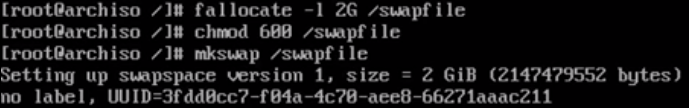
\includegraphics[width=0.7\textwidth]{./figures/swapfile.png}
  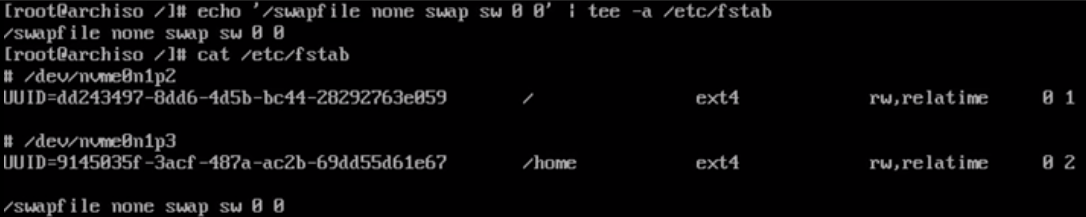
\includegraphics[width=\textwidth]{./figures/swapfile2.png}
\end{frame}

\begin{frame}[fragile]{Finish}
  \begin{itemize}
    \item \inlinebox{exit}, to exit out of chroot
    \item \inlinebox{umount -R /mnt}
      \item \inlinebox{umount -l /mnt} (to force unmount) or \inlinebox{umount -a}
    \item \inlinebox{poweroff} (not \inlinebox{reboot} to remove the iso from storage in virtualbox)
    \item in the UFEI firmware settings   choose the right bootloader for the esp on which the bootloader was installed (maybe secure boot has to be enabled for this) and give the esp with the bootloader the highest boot priority
  \end{itemize}
\end{frame}

\section{NixOs Base Installation}

\begin{frame}[fragile]{Dualbooting with Windows 11}
  \centering
  \begin{terminal}[minted language=nix]
    # boot.loader.systemd-boot.enable = true;
    boot.loader.efi.canTouchEfiVariables = true;
    boot.loader.grub.enable = true;
    boot.loader.grub.devices = [ "nodev" ];
    boot.loader.grub.efiSupport = true;
    boot.loader.grub.use0SProber = true;
  \end{terminal}
  \begin{itemize}
  \item \url{https://www.youtube.com/watch?v=82vrj22omyQ&list=PLXJMLVnWDKP0KQc1kbGbgyCz90yuecKKm&index=2&t=319s}
  \end{itemize}
\end{frame}

\begin{frame}[fragile]{Labeling}
  \begin{itemize}
    \item \inlinebox*{e2label /dev/XXX "new label"}
    \item \inlinebox*{swaplabel -L "new label" /dev/XXX}
    \item \inlinebox*{fatlabel /dev/XXX "new label"}
    \item \url{https://wiki.archlinux.org/title/Persistent_block_device_naming}
  \end{itemize}
\end{frame}

% \begin{frame}[fragile]{}{}
%   \begin{itemize}
%
%   \end{itemize}
% \end{frame}

%!Tex Root = ../Linux_Installation.tex
% ./content_Linux_Installation/Packete
% ./content_Linux_Installation/Design
% ./content_Linux_Installation/Deklarationen
% ./content_Linux_Installation/Before_Installation
% ./content_Linux_Installation/Base_Installation

\section{Arch Linux After Base Installation}

\begin{frame}[fragile]{General}
  \begin{itemize}
    \item if one forgot one step in the base installation with \inlinebox{su}, one can get root again.
    \item {\tiny\inlinebox{sudo pacman -S base-devel, xorg-xkill, man-db texinfo openssh e2fsprogs, dialog}}: \inlinebox{base-devel} is for building aur packages and \inlinebox{sudo} and \inlinebox{which} are in there, enable \inlinebox{openssh} with \inlinebox{systemsctl enable sshd}, \inlinebox{dialog} is a cli-textbox some programs use.
    \item if sth. goes wrong with the DE one can change tty with \inlinebox{ctrl + alt + fX} and make e.g. \inlinebox{killall i3}.
  \end{itemize}
\end{frame}

\begin{frame}[fragile, allowframebreaks]{Desktop-Environment / WM\vspace{0.5cm}}
  \begin{itemize}
    \item \inlinebox{sudo pacman -S xorg-server xorg-xinit}
    \item \alert{i3:}
      \begin{itemize}
        \item \inlinebox{sudo pacman -S i3-gaps i3status alacritty dmenu}
        \item install fonts (i3 doesn't pull fonts), e.g. \inlinebox{sudo pacman -S noto-fonts}
      \end{itemize}
    \item \alert{xfce:}
      \begin{itemize}
        \item \inlinebox{sudo pacman -S xfce4, xfce4-goodies, lightdm, lightdm-gtk-greeter}, \inlinebox{systemctl enable lightdm}
      \end{itemize}
    \item \alert{gnome:} \inlinebox{pacman -S gnome}, \inlinebox{gnome-tweaks}, \inlinebox{systemctl enable gdm}
    \item \alert{kde:}  \inlinebox{plasma-meta}, \inlinebox{kde-applications}, \inlinebox{systemctl enable sddm}
    \item \inlinebox{cp /etc/X11/xinit/xinitrc /home/areo/.xinitrc}
    \item \inlinebox{nvim ~/.xinitrc}: write \inlinebox{exex i3} or \inlinebox{exec xfce4-session} in there
    \item \inlinebox{startx} to start
    \item \inlinebox{xrandr} to show all available screen resolutions and then e.g. \inlinebox{xrandr -s 1920x780}
  \end{itemize}
\end{frame}

\begin{frame}[fragile]{Start DE directly after login or set up a display manager (login screen)}
  \begin{itemize}
    \item \inlinebox{~/.zshrc} or \inlinebox{~/.bash_profile}:
      \begin{terminal}[minted language=bash]
        if [[ "$(tty)" = "/dev/tty1" ]]; then
          pgrep || startx
        fi
      \end{terminal}
    \item \alert{displaymanager:}
      \begin{itemize}
        \item \inlinebox{sudo pacman -S lightdm lightdm-gtk-greeter}
        \item \inlinebox{sudo systemctl enable lightdm.service}: systemd command to tell systemd to start lightdm when one does log in
        \item useful to be able to choose between differnt desktop environments
      \end{itemize}
  \end{itemize}
\end{frame}

\begin{frame}[fragile]{Compiling yay (make arch package)}
  \begin{itemize}
    \item \inlinebox{git clone https://aur.archlinux.org/yay-git.git}
    \item \inlinebox{cd yay-git} and then \inlinebox{makepkg -si}
      \begin{itemize}
        \item \inlinebox{base-devel} needed for it
      \end{itemize}
  \end{itemize}
\end{frame}

\begin{frame}[fragile]{Arch in Virtualbox (in case)}
  \begin{itemize}
    \item \inlinebox{pacman -S virtualbox-guest-utils xf86-video-vmware}
  \end{itemize}
\end{frame}

\begin{frame}[fragile]{Wifi}
  \begin{itemize}
    \item NetworkManager manages everything ones it is activated (ethernet an wifi)
      \item \inlinebox{wifi-menu} doesn't work once the NetworkManager is activated or if there's already a ethernet connection
    \item \inlinebox{nmcli device wifi list}
    \item {\tiny \inlinebox{nmcli device wifi connect 'FRITZ!Box Gastzugang Herbert' password PASSWORD}}
  \end{itemize}
\end{frame}

\begin{frame}[fragile]{CPU/GPU}
  \begin{itemize}
    \item \alert{Microcode:} \inlinebox{pacman -S amd-ucode} or \inlinebox{pacman -S intel-ucode}
    \item \inlinebox{pacman -S xf86-video-intel}
    \item \inlinebox{pacman -S mesa} (if intel or amd for graphics) or \inlinebox{pacman -S nvidea nvidea-utils} (nvideo for graphics) and \inlinebox{pacman -S nvidea-lts} (if one installed the lts-kernel)
    \item \inlinebox{pacman -S virtualbox-guest-utils xf86-video-vmware} and \inlinebox{systemctl enable vboxservice}(if in Virtualbox)
  \end{itemize}
\end{frame}

\begin{frame}[fragile,allowframebreaks]{Right Keyboard Layout in Xorg\vspace{0.5cm}}
  \begin{itemize}
    \item for xorg the keyboard layout isn't related to the keyboard layout in the tty with it's file: \inlinebox{/etc/vconsole.conf} but has to be configured in e.g. \inlinebox{/etc/X11/xorg.conf.d/00-keyboard.conf} (one of many keyboard layouts for xorg)
      \begin{itemize}
        \item xorg.conf is parsed by the X server at start-up. To apply changes, restart X
      \end{itemize}
    \item \alert{get overview:}
      \begin{terminal}[minted language=bash]
        localectl list\itemx11-keymap-models
        localectl list\itemx11-keymap-layouts
        localectl list\itemx11-keymap-variants [layout] (e.g. de)
        localectl list\itemx11-keymap-options
      \end{terminal}
  \item set one for the current session: \inlinebox{sudo setxkbmap de nodeadkeys} or \inlinebox{sudo setxkbmap -layout de -variant nodeadkeys} (long variant)
    \begin{itemize}
      \item {\tiny \inlinebox{setxkbmap [-model xkb_model] [-layout xkb_layout] [-variant xkb_variant] [-option xkb_options]}}
      \item or persistent in \inlinebox{~/.xinitrc}
    \end{itemize}
  \item make persistent in \inlinebox{/etc/X11/xorg.conf.d}:
    \begin{itemize}
      \item \inlinebox{localectl set-x11-keymap de "" nodeadkeys ""}: autogenerates the keyboard layout file
      \item {\tiny \inlinebox{localectl [--no-convert] set-x11-keymap layout [model [variant [options]]]}}
      \item if \inlinebox{--no-convert} option is passed, the specified keymap is also converted to the closest matching console keymap and applied to the console configuration in \inlinebox{vconsole.conf}
      \item to set a model, variant or options, all preceding fields need to be specified, but the preceding fields can be skipped by passing an empty string with ""
    \end{itemize}
  \end{itemize}
\end{frame}

\begin{frame}[fragile]{Desktop Background}
  \begin{itemize}
    \item {\tiny \inlinebox{feh --bg-scale "/home/areo/Pictures/Wallpaper/linux wallpaper/urban-1597922375998-8560.jpg"}}
    \begin{itemize}
      \item best into \inlinebox{~/.xinitrc}
    \end{itemize}
  \end{itemize}
\end{frame}

\begin{frame}[fragile]{Sound}
  \begin{itemize}
    \item \inlinebox{sudo pacman -S pulseaudio}
    \item \inlinebox{/usr/bin/start-pulseaudio-x11}
    \begin{itemize}
      \item best into \inlinebox{~/.xinitrc}
    \end{itemize}
    \item \inlinebox{pavucontrol} is a gui to have an overview
  \end{itemize}
\end{frame}

\begin{frame}[fragile]{Compositor}
  \begin{itemize}
    \item \inlinebox{picom &}
      \begin{itemize}
        \item best into \inlinebox{~/.xinitrc}
      \end{itemize}
  \end{itemize}
\end{frame}

\begin{frame}[fragile]{Screen-Brightness}
  \begin{itemize}
    \item \inlinebox{sys/class/backlight}
  \end{itemize}
\end{frame}

\begin{frame}[fragile]{Screenshot}
  \begin{itemize}
    \item \inlinebox{scrot} ($\rightarrow$ configuration in \inlinebox{~/.config/i3/config} file)
  \end{itemize}
\end{frame}

\begin{frame}[fragile]{SysRq-Key einsetzen}
  \begin{itemize}
    \item \alert{reboot:} \key{alt} + \key{print} + each of \smalltt{reisub}.
    \item \alert{shut down:} \key{alt} + \key{print} + each of \smalltt{reisuo}.
    \item Bedeutung der Keys kann hier nachgelesen werden: \url{https://en.wikipedia.org/wiki/Magic_SysRq_key}.
    % \item https://en.wikipedia.org/wiki/Magic_SysRq_key
  \end{itemize}
  \begin{Sidenote}
    \begin{itemize}
      \item Nach dem Auslösen von e sollte man den Prozessen ein paar Sekunden Zeit lassen, der Aufforderung, sich sauber zu beenden, nachzukommen.
      \item SysRq may be released before pressing the command key, as long as Alt remains held down.
      \item this keys are for the querty keyboard.
    \end{itemize}
  \end{Sidenote}
\end{frame}

\begin{frame}[fragile]{SysRq-Key aktivieren}
  \begin{itemize}
    \item \alert{direkt aktivieren, aber nicht persistent} {\tiny \inlinebox{echo "1" | sudo tee /proc/sys/kernel/sysrq}}.
    \item \alert{persistent aktivieren} {\tiny \inlinebox*{echo kernel.sysrq=1 | sudo tee /etc/sysctl.d/99-sysctl.conf}.}
  \end{itemize}
  % \item https://linuxconfig.org/how-to-enable-all-sysrq-functions-on-linux
  % \item https://archived.forum.manjaro.org/t/how-to-permanently-enable-the-sysrq-key/137650/6
  \begin{Sidenote}
    \begin{itemize}
      \scriptsize
      \item \alert{geht auch:} {\tiny {\tiny \inlinebox*{sudo bash -c "echo kernel.sysrq=1 > /etc/sysctl.d/99-sysctl.conf"}}}.
      \item {\tiny \inlineboxsout*{sudo echo "kernel.sysrq=1" > /etc/sysctl.d/99-sysctl.conf}}.
      \begin{itemize}
        \item The reason it doesn't work is that ones gives root privileges to echo, which it doesn't need to print to stdout. It's bash doing the writing to file and that's running under your user.
      \end{itemize}
      \item \inlinebox{tee -a} or \inlinebox{>>} for appending.
    \end{itemize}
  \end{Sidenote}
\end{frame}

\begin{frame}[fragile, t]{SysRq-Key checken}
  % , squeeze
  \begin{columns}
    \begin{column}[t]{0.5\textwidth}
      \begin{itemize}
        \item \inlinebox{cat /proc/sys/kernel/sysrq}
          \begin{itemize}
            \item 0 - disable sysrq completely.
            \item 1 - enable all functions of sysrq.
            \item 2 - enable control of console logging level.
            \item 4 - enable control of keyboard (SAK, unraw).
            \item 8 - enable debugging dumps of processes etc.
            \item 16 - enable sync command.
            \item 32 - enable remount read-only.
            \item 64 - enable signaling of processes (term, kill, oom-kill).
          \end{itemize}
      \end{itemize}
    \end{column}
    \begin{column}[t]{0.5\textwidth}
      \begin{itemize}
        \item 128 - allow reboot/poweroff.
        \item 256 - allow nicing of all RT tasks.
      \end{itemize}
      \vspace{0.3cm}
      \begin{Sidenote}
        \begin{itemize}
         \scriptsize
          \item 438 is obtained from the sum of 2 + 4 + 16 + 32 + 128 + 256, so all the corresponding functions are enabled.
        \end{itemize}
      \end{Sidenote}
    \end{column}
  \end{columns}
\end{frame}

\begin{frame}[fragile]{Restore boobtable USB-Stick to normal}{Explanation}
  \begin{itemize}
    \item if one writes a iso-image onto a flash drive there're e.g 2 partitions encoded in the iso image and a lot of free space.
    \item if one writes a iso to the flash drive, it will get a \alert{boot flag} (that can be seen with \inlinebox{sudo fdisk -l}. If one only formats it, it won't work correctly (can't remove partitions etc.).
    \item one has to wipe filesystem completely from the flash drive, to restore it to it's original state.
  \end{itemize}
\end{frame}

\begin{frame}[fragile, allowframebreaks]{Restore boobtable USB-Stick to normal}{Format / repartition a storage device\vspace{0.5cm}}
  \begin{itemize}
    \item \inlinebox{sudo fdisk -l}
    \item \inlinebox{lsblk -o NAME,FSTYPE,SIZE,MOUNTPOINT,LABEL}
    \item \inlinebox{sudo wipefs --all /dev/sdc}
    \begin{itemize}
      \item whole drive, not \inlinebox{sdc1}!
    \end{itemize}
    \item \inlinebox{sudo cfdisk /dev/sdc}
      \begin{itemize}
        \item GPT wählen
        \item DOS ist eine andere Bezeichnung für MBR
      \end{itemize}
    \item \inlinebox{sudo mkfs.ext4 /dev/sdc1}
      \begin{itemize}
        \item \inlinebox{-n 'My_USB'} to give it a name
      \end{itemize}
    \item \inlinebox{sudo chmod 755 . -R}
    \item \inlinebox{sudo chown areo:users . -R}
  \end{itemize}
  \begin{Sidenote}
    \begin{itemize}
      \item need to \inlinebox{sudo umount /dev/sdX} flash drive before \inlinebox{wipefs} / \inlinebox{mkfs.vfat} etc.
    \end{itemize}
  \end{Sidenote}
\end{frame}


\section{Literatur}

\begin{frame}{Bücher}
  \printbibliography[type=book,heading=subbibliography,title={Bücher}]
\end{frame}

\begin{frame}{Artikel}
  \printbibliography[type=article,heading=subbibliography,title={Artikel}]
\end{frame}

\begin{frame}{Vorlesungen}
  \printbibliography[type=unpublished,heading=subbibliography,title={Vorlesungen}]
\end{frame}

\begin{frame}{Online}
  \printbibliography[type=online,heading=subbibliography,title={Online}]
\end{frame}

\begin{frame}{Sonstiges}
  \printbibliography[nottype=book, nottype=article, nottype=online, nottype=unpublished,heading=subbibliography,keyword=wikikeyword,title={Sonstige Quellen}]
\end{frame}
\end{document}
